\cchapter{Introduction}

Computational visualization of large molecules -- particularly for
protein and RNA structures -- has gained tremendous importance as a
cutting-edge tool for biological research.  Previous work has
focused on efficient rendering for single-component, static
molecules, which is becoming increasingly restricted in light of the
increasing demand for more complex, dynamic visualization and
representation.  We present \TexMol (short for Texture Molecular
Viewer), an interactive molecular exploration package created in
response to the increasingly demanding visualization needs of the
biology community.

To efficiently visualize dynamic and flexible structures, \TexMol
uses a molecular specification file to construct the Flexible Chain
Complex (FCC), a robust, dynamic data structure that serves as
\TexMol's internal representation for molecular structures.  The FCC
models the flexible joints of a molecule and contains a
biochemically-based hierarchy for level-of-detail optimizations.

Besides high visualizer functionality, \TexMol delivers rapid,
accurate rendering via various novel applications of texture-based
rendering techniques for structural and for volumetric
representations.  For the field of structural representation (e.g.
CPK (of union of balls, where each atom is represented by a sphere
with the radius equal to the van der Waals radius.), ball-and-stick
model), recent advances in programmable graphics hardware have
opened the door for texture-based rendering -- also known as
imposter rendering -- that greatly reduces geometric complexity
while preserving, and in some cases improving the visual fidelity of
the final image. \TexMol's level-of-detail hierarchy allows for
static and dynamic multiresolution, which reduces the visual clutter
that often accompanies atom-level visualization while still
maintaining biochemical structural information, such as
residue-level grouping.  Combined with the level-of-detail
hierarchy, texture-based rendering allows \TexMol to render large
and previously intractable molecules.

\TexMol also supports efficient volumetric visualization via
texture-based techniques. By combining rendering modes, the
visualizer can either map volumetric data onto the structural model
of the molecule or it can juxtapose multiple volume sets and
structure models concurrently. In both cases, the resulting
visualization ties molecular structure to molecular function in an
elucidating manner.

\csection{Functions} \TexMol is both a visualization and
computational toolkit for large biomolecules. Some of the main
features include

\begin{itemize}

\item Open source software for rendering large molecule data sets.
It has been tested on molecules with more than 3million atoms.

\item Written in C++, with a QT front end. The same code should work
on multiple platforms, including Windows and Linux.

\item Reads in the well known PDB and PQR formats.

\item Produces high quality images using High-end graphics cards
functionalities.

\item Volume rendering and calculation of electron density,
hydrophobicity functions.

\item Wireframe and smooth shaded isosurfaces.

\item Computes metrics including curvatures, surface areas and
volumes.

\item Provides programmers with a simple and yet powerful hierarchical
data structure of the molecules, with various torsion angles
calculated.

\item Multiple views and multiple data set rendering.

\end{itemize}

\csection{Installation}

Please install \TexMol and perform the functions described in the
rest of the tutorial to learn more about the software. \TexMol is
open source and should be available for download from CCV's software
download page. It has been tested under both windows and linux. You
will need the following

\begin{itemize}

\item A windows or linux operating system.

\item QT and a C++ compiler.

\item A high end graphics card, like GeForce fx or better.

\item An input PDB file, which can be downloaded off the PDB
database.

\end{itemize}

Once you have downloaded the source, you can compile it using either
the QT's Makefiles (the .pro files) or the project workspace files
(for windows).

\subsection{Step by step installation guide}

There are some subtle problems which could come up when compiling
and linking \TexMol. Here are some solutions.

\begin{itemize}

\item Check to ensure that you have a good graphics card. We have
currently tested our programs on NVidia's cards, GeForce fx and
beyond.

\item Upgrade your graphics card drivers and test example Cg
programs they usually provide. There should be examples on NVidia's
website, which can help you ensure that it is set up well.

\item Make sure that the latest Cg compiler is installed.

\item Define the environment variables CG\_BIN\_PATH, CG\_LIB\_PATH and
CG\_INC\_PATH if it was not already done.

\item Download and install QT. There is a free version for Linux.

\item Make sure that the variables QTDIR and QTLIB are defined.

\item If the contour library is being used, the user, unfortunately
needs to define whether they are using a big endian or little endian
machine. Hence, you may or may not need to define the variable
LITTLE\_ENDIAN. Other libraries do not need this and can figure out
the endianness in the code.

\end{itemize}

\subsection{Common installation problems}

\begin{itemize}

\item Compilation problems

    \begin{itemize}

    \item \emph{QT and X11 incompatibility}

    You could get into problems due to QT and X11 defining things arbitrarily.
    One way to get around this is to change some
    headers or redefine the error causing terms.

    \item \emph{Gl extensions}

    Download the latest glext.h from SGI's website. DELETE other vendors
    glext.h. Before installing
    \TexMol, check to see if Gl and Cg demos are working.

    \item \emph{file not found}

    QT's internal compilers may not have created the files needed by a
    library in a subfolder of \TexMol. Try compiling a different
    subfolder or the main folder itself and try again.

    \end{itemize}

\item Rendering issues

    \begin{itemize}

    \item \emph{Doesn't render}

    Cg files provided are linked in at run time. So you will need to
    keep them in the same folder as \TexMol's executable.

    \end{itemize}

\end{itemize}

\csection{The main user interface}

In figure \ref{figure:userInterface}, we show a volume rendering and
isosurface of a molecule. The different regions in the user
interface are

\begin{figure}
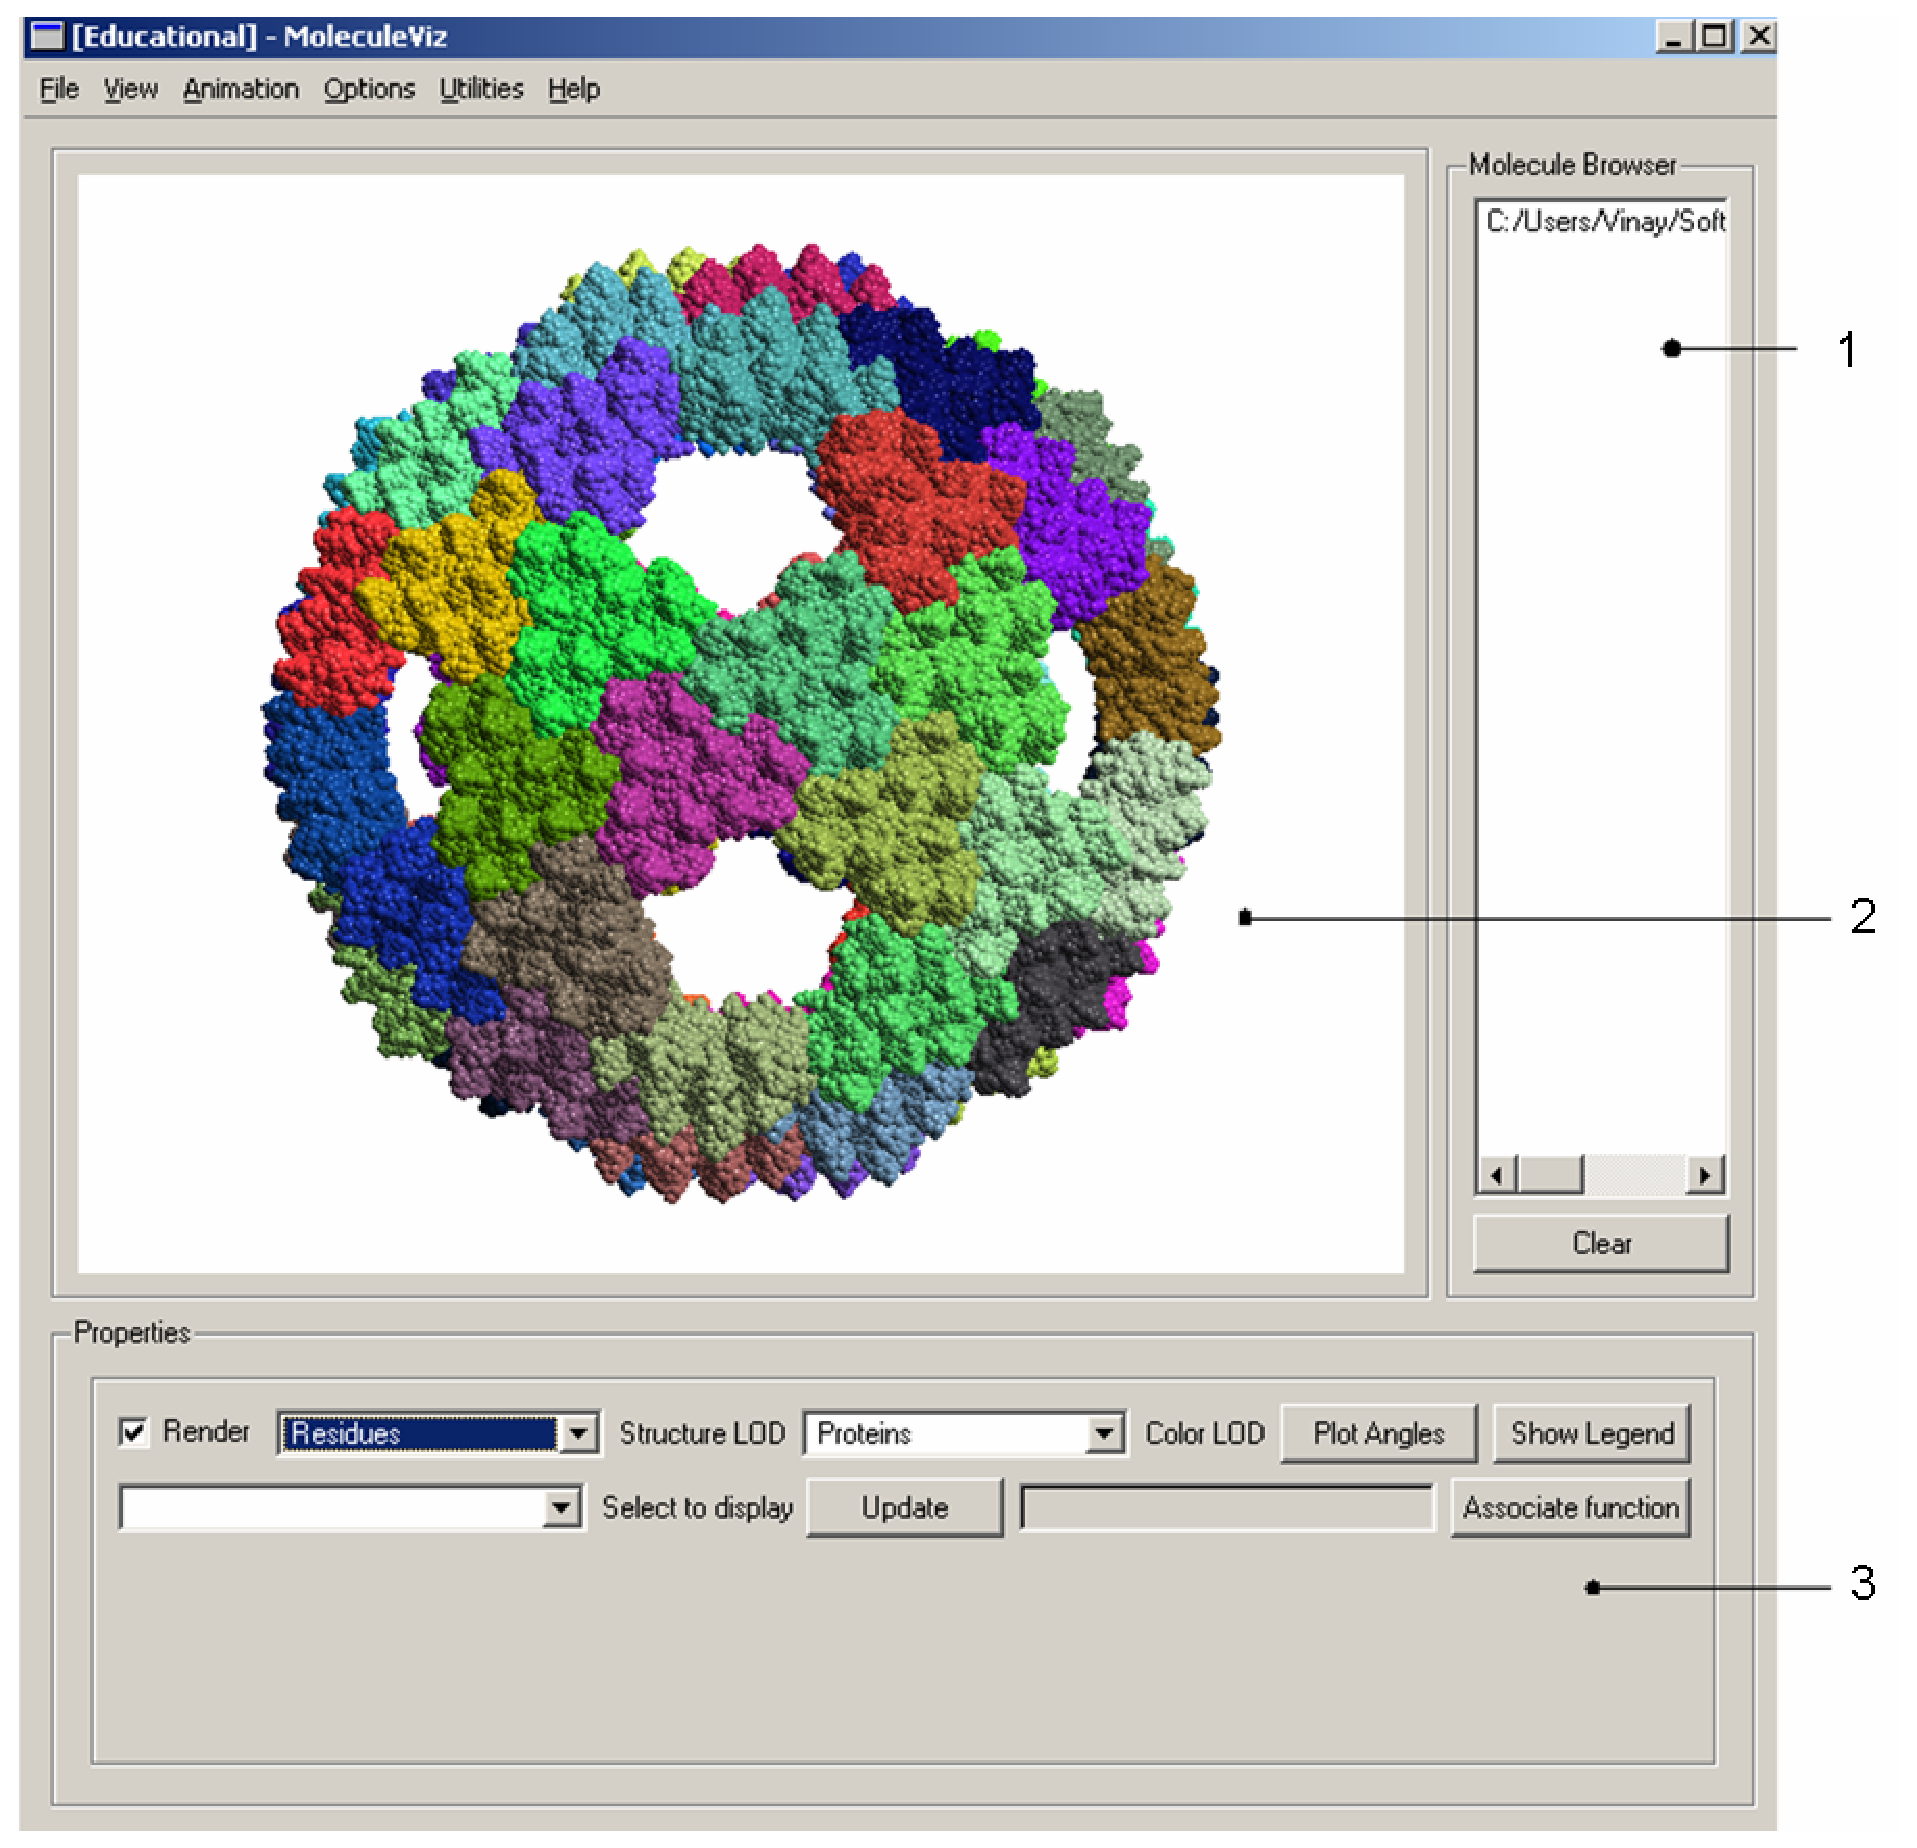
\includegraphics[width=5in]{Images/UserInterface.ps}
\ccaption{The main user interface of \TexMol. In this figure, we
mark the three main regions users should get familiar with: 1.
\emph{Molecule browser} where data sets names are displayed 2.
\emph{Rendering area}, where data is rendered and 3. The
\emph{Properties widget} where the properties of the selected data
set is shown.} \label{figure:userInterface}
\end{figure}

\begin{itemize}

\item Molecule browser. The list of molecules are shown here. The
name is displayed, and if it was left blank on opening the file, the
full filename is shown. The user can select files to either
manipulate it using the properties window or to delete it.

\item The rendering area. This is either in perspective or
orthographic mode, runs using OpenGL and can be either a single or
multiple views.

\item Properties area. Each type of file  (volume, molecule or
surface) has its own unique properties widget which is displayed
here. On selecting a data set from the browser, its corresponding
properties are displayed here.

\end{itemize}
